\chapter{Resultados}
Os resultados seguem o metodo de \citeonline{raman1928} e \citeonline{feynman1965}.
\section{Sistema de equacoes}
\begin{align}
a &= b + c \\
d &= e - f
\end{align}
Os valores aparecem na Tabela~\ref{tab:dois} e na Figura~\ref{fig:dois}.
\begin{figure}[htb]
\caption{Desenho vetorial dois}\label{fig:dois}
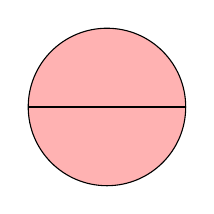
\begin{tikzpicture}\draw[fill=red!30] (0,0) circle (1);\draw (-1,0) -- (1,0);\end{tikzpicture}
\end{figure}
\begin{table}[htb]
\caption{Tabela de resultados dois}\label{tab:dois}
\begin{tabular}{lcc}\hline
Ensaio & Tempo & Erro \\ \hline
um & 10 & 0 \\
dois & 20 & 1 \\ \hline
\end{tabular}
\end{table}
\section{Discussao}
A discussao compara os dois ensaios e conclui que o erro cresce com o tempo.
\chapter{Conclusao}
O trabalho conclui que a exportacao precisa manter a estrutura do documento.
